\documentclass{article}

\usepackage{fancyhdr}
\usepackage{extramarks}
\usepackage{amsmath}
\usepackage{amsthm}
\usepackage{amsfonts}
\usepackage{amssymb}
\usepackage{xparse}
\usepackage{tikz}
\usepackage{graphicx}
\usepackage[plain]{algorithm}
\usepackage{algpseudocode}
\usepackage{listings}
\usepackage{hyperref}
\usepackage[per-mode = fraction]{siunitx}
\usepackage{calc}

\usetikzlibrary{automata,positioning}

\hypersetup{
    colorlinks=true,
    linkcolor=blue,
    filecolor=magenta,
    urlcolor=blue,
    }

\urlstyle{same}

%
% Basic Document Settings
%

\topmargin=-0.45in
\evensidemargin=0in
\oddsidemargin=0in
\textwidth=6.5in
\textheight=9.0in
\headsep=0.25in

\linespread{1.1}

\pagestyle{fancy}
\lhead{\hmwkAuthorName}
\chead{\hmwkClass\ (\hmwkClassInstructor,\ \hmwkClassTime): \hmwkTitle}
\rhead{\firstxmark}
\lfoot{\lastxmark}
\cfoot{\thepage}

\renewcommand\headrulewidth{0.4pt}
\renewcommand\footrulewidth{0.4pt}

\setlength\parindent{0pt}
\allowdisplaybreaks
%
% Title Page
%

\title{
	\vspace{2in}
	\textmd{\textbf{\hmwkClass:\ \hmwkTitle}}\\
	\normalsize\vspace{0.1in}\small{Due\ on\ \hmwkDueDate\ at \hmwkDueTime}\\
	\vspace{0.1in}\large{\textit{\hmwkClassInstructor,\ \hmwkClassTime}}
	\vspace{3in}
}
\author{\textbf{\hmwkAuthorName}}
\date{\hmwkCompletionDate}

%
% Create Problem Sections
%

\newcommand{\enterProblemHeader}[1]{
	\nobreak\extramarks{}{Problem #1 continued on next page\ldots}\nobreak{}
	\nobreak\extramarks{Problem #1 (continued)}{Problem #1 continued on next page\ldots}\nobreak{}
}

\newcommand{\exitProblemHeader}[1]{
	\nobreak\extramarks{Problem #1 (continued)}{Problem #1 continued on next page\ldots}\nobreak{}
	\nobreak\extramarks{Problem #1}{}\nobreak{}
}

%
% Homework Problem Environment
%
\NewDocumentEnvironment{hwkProblem}{m m s}{
	\section*{Problem #1: #2}
	\enterProblemHeader{#1}
	\setcounter{partCounter}{1}
}{
	\exitProblemHeader{#1}
	\IfBooleanF{#3} % if star, no new page
		{\newpage}
}

% Alias for the Solution section header
\newcommand{\hwkSol}{\vspace{\baselineskip / 2}\textbf{\Large Solution}\vspace{\baselineskip / 2}}

% Alias for the Solution Part subsection header
\newcounter{partCounter}
\newcommand{\hwkPart}{
	\vspace{\baselineskip / 2}
	\textbf{\large Part \Alph{partCounter}}
	\vspace{\baselineskip / 2}
	\stepcounter{partCounter}
}

%
% Various Helper Commands
%

% Such That
\newcommand{\st}{\text{s.t.}}

% Useful for algorithms
\newcommand{\alg}[1]{\textsc{\bfseries \footnotesize #1}}

% For derivatives
\newcommand{\deriv}[1]{\frac{\mathrm{d}}{\mathrm{d}x} (#1)}

% For partial derivatives
\newcommand{\pderiv}[2]{\frac{\partial}{\partial #1} (#2)}

% Integral dx
\newcommand{\dx}{\mathrm{d}x}
\newcommand{\dy}{\mathrm{d}y}

% Probability commands: Expectation, Variance, Covariance, Bias
\newcommand{\e}[1]{\mathrm{e}#1}
\newcommand{\E}{\mathrm{E}}
\newcommand{\Var}{\mathrm{Var}}
\newcommand{\Cov}{\mathrm{Cov}}
\newcommand{\Bias}{\mathrm{Bias}}

% Defining Units that are not in the SI base
\DeclareSIUnit\bar{bar}
\DeclareSIUnit\ft{ft}
\DeclareSIUnit\dollar{\$}
\DeclareSIUnit\cent{\text{\textcent}}
\DeclareSIUnit\c{\degreeCelsius}

% Code Listing config
\usepackage{xcolor}
\definecolor{codegreen}{rgb}{0,0.6,0}
\definecolor{codegray}{rgb}{0.5,0.5,0.5}
\definecolor{codepurple}{rgb}{0.58,0,0.82}
\definecolor{backcolour}{rgb}{0.95,0.95,0.92}
\lstdefinestyle{overleaf}{
	% backgroundcolor=\color{backcolour},
	commentstyle=\color{codegreen},
	keywordstyle=\color{magenta},
	numberstyle=\tiny\color{codegray},
	stringstyle=\color{codepurple},
	basicstyle=\ttfamily\footnotesize,
	breakatwhitespace=false,
	breaklines=true,
	captionpos=b,
	keepspaces=true,
	numbers=left,
	numbersep=5pt,
	showspaces=false,
	showstringspaces=false,
	showtabs=false,
	tabsize=4
}

\usepackage[latte]{catppuccinpalette}
\lstdefinestyle{catppuccin}{
	breaklines=true,
	keepspaces=true,
	numbers=left,
	numbersep=5pt,
	showspaces=false,
	showstringspaces=false,
	breakatwhitespace=true,
	tabsize=4,
	stringstyle = {\color{CtpGreen}},
	commentstyle={\color{CtpOverlay1}},
	basicstyle = {\small\color{CtpText}\ttfamily},
	keywordstyle = {\color{CtpMauve}},
	keywordstyle = [2]{\color{CtpBlue}},
	keywordstyle = [3]{\color{CtpYellow}},
	keywordstyle = [4]{\color{CtpLavender}},
	keywordstyle = [5]{\color{CtpPeach}},
	keywordstyle = [6]{\color{CtpTeal}}
}

\lstset{style=catppuccin}

% chktex-file 8

%
% Homework Details
%   - Title
%   - Subtitle
%   - Due date
%   - Due time
%   - Course
%   - Section/Time
%   - Instructor
%   - Author
%

\newcommand{\hmwkTitle}{Homework 05}
\newcommand{\hmwkSubTitle}{MATLAB \& Transfer Functions}
\newcommand{\hmwkDueDate}{March 7th, 2025}
\newcommand{\hmwkDueTime}{05:00 PM}
\newcommand{\hmwkClass}{ENAE 432  0101}
\newcommand{\hmwkClassTime}{09:00}
\newcommand{\hmwkClassInstructor}{Dr.\ Sanner}
\newcommand{\hmwkAuthorName}{\textbf{Vai Srivastava}}
\newcommand{\hmwkCompletionDate}{\today}

\begin{document}

\maketitle

\pagebreak

\begin{hwkProblem}{1}{}

	Consider the family of transfer functions: \[ \func{G}[s] = \frac{6 \left(\tau s + 1\right)}{s^{2} + 2s + 4}. \]
	\begin{enumerate}
		\item Use Matlab to generate the step response for this system in the three cases \(\tau=0\), \(\tau=1\), and \(\tau=-1\). Use hold on to overlay all three responses on a single graph. Rightclick on the resulting plot and use the "Characteristics" submenu to label the peak values and times. Click on the dots that appear to pop up a box with numerical details about each point.
		\item Qualitatively, how do the responses in P01a agree with the class discussion regarding step responses for transfer functions containing zeros? Quantitatively, how do the numerical values for peak response and peak time agree with the class discussion in the specific case that \(\tau=0\) ?
	\end{enumerate}

	\hwkSol{}

	\begin{lstlisting}[language={matlab}, label={lst:s01}, caption={MATLAB code for HW05 P01}]
		s = tf('s');
		tau = [0, 1, -1];
		colors = ['r', 'b', 'g'];
		denom = s^2 + 2*s + 4;

		figure;
		hold on;
		for j = 1:length(tau)
			G = 6 * (tau(j) * s + 1) / denom;
			step(G,colors(j));
		end

		grid on;
		legend('\tau = 0', '\tau = 1', '\tau = -1', Location="southeast");
		title('Step Response of \tau');
		xlabel('Time');
		ylabel('Response');
		hold off;
	\end{lstlisting}

	\hwkPart{}

	Part A answer

	\begin{figure}[H]
		\begin{center}
			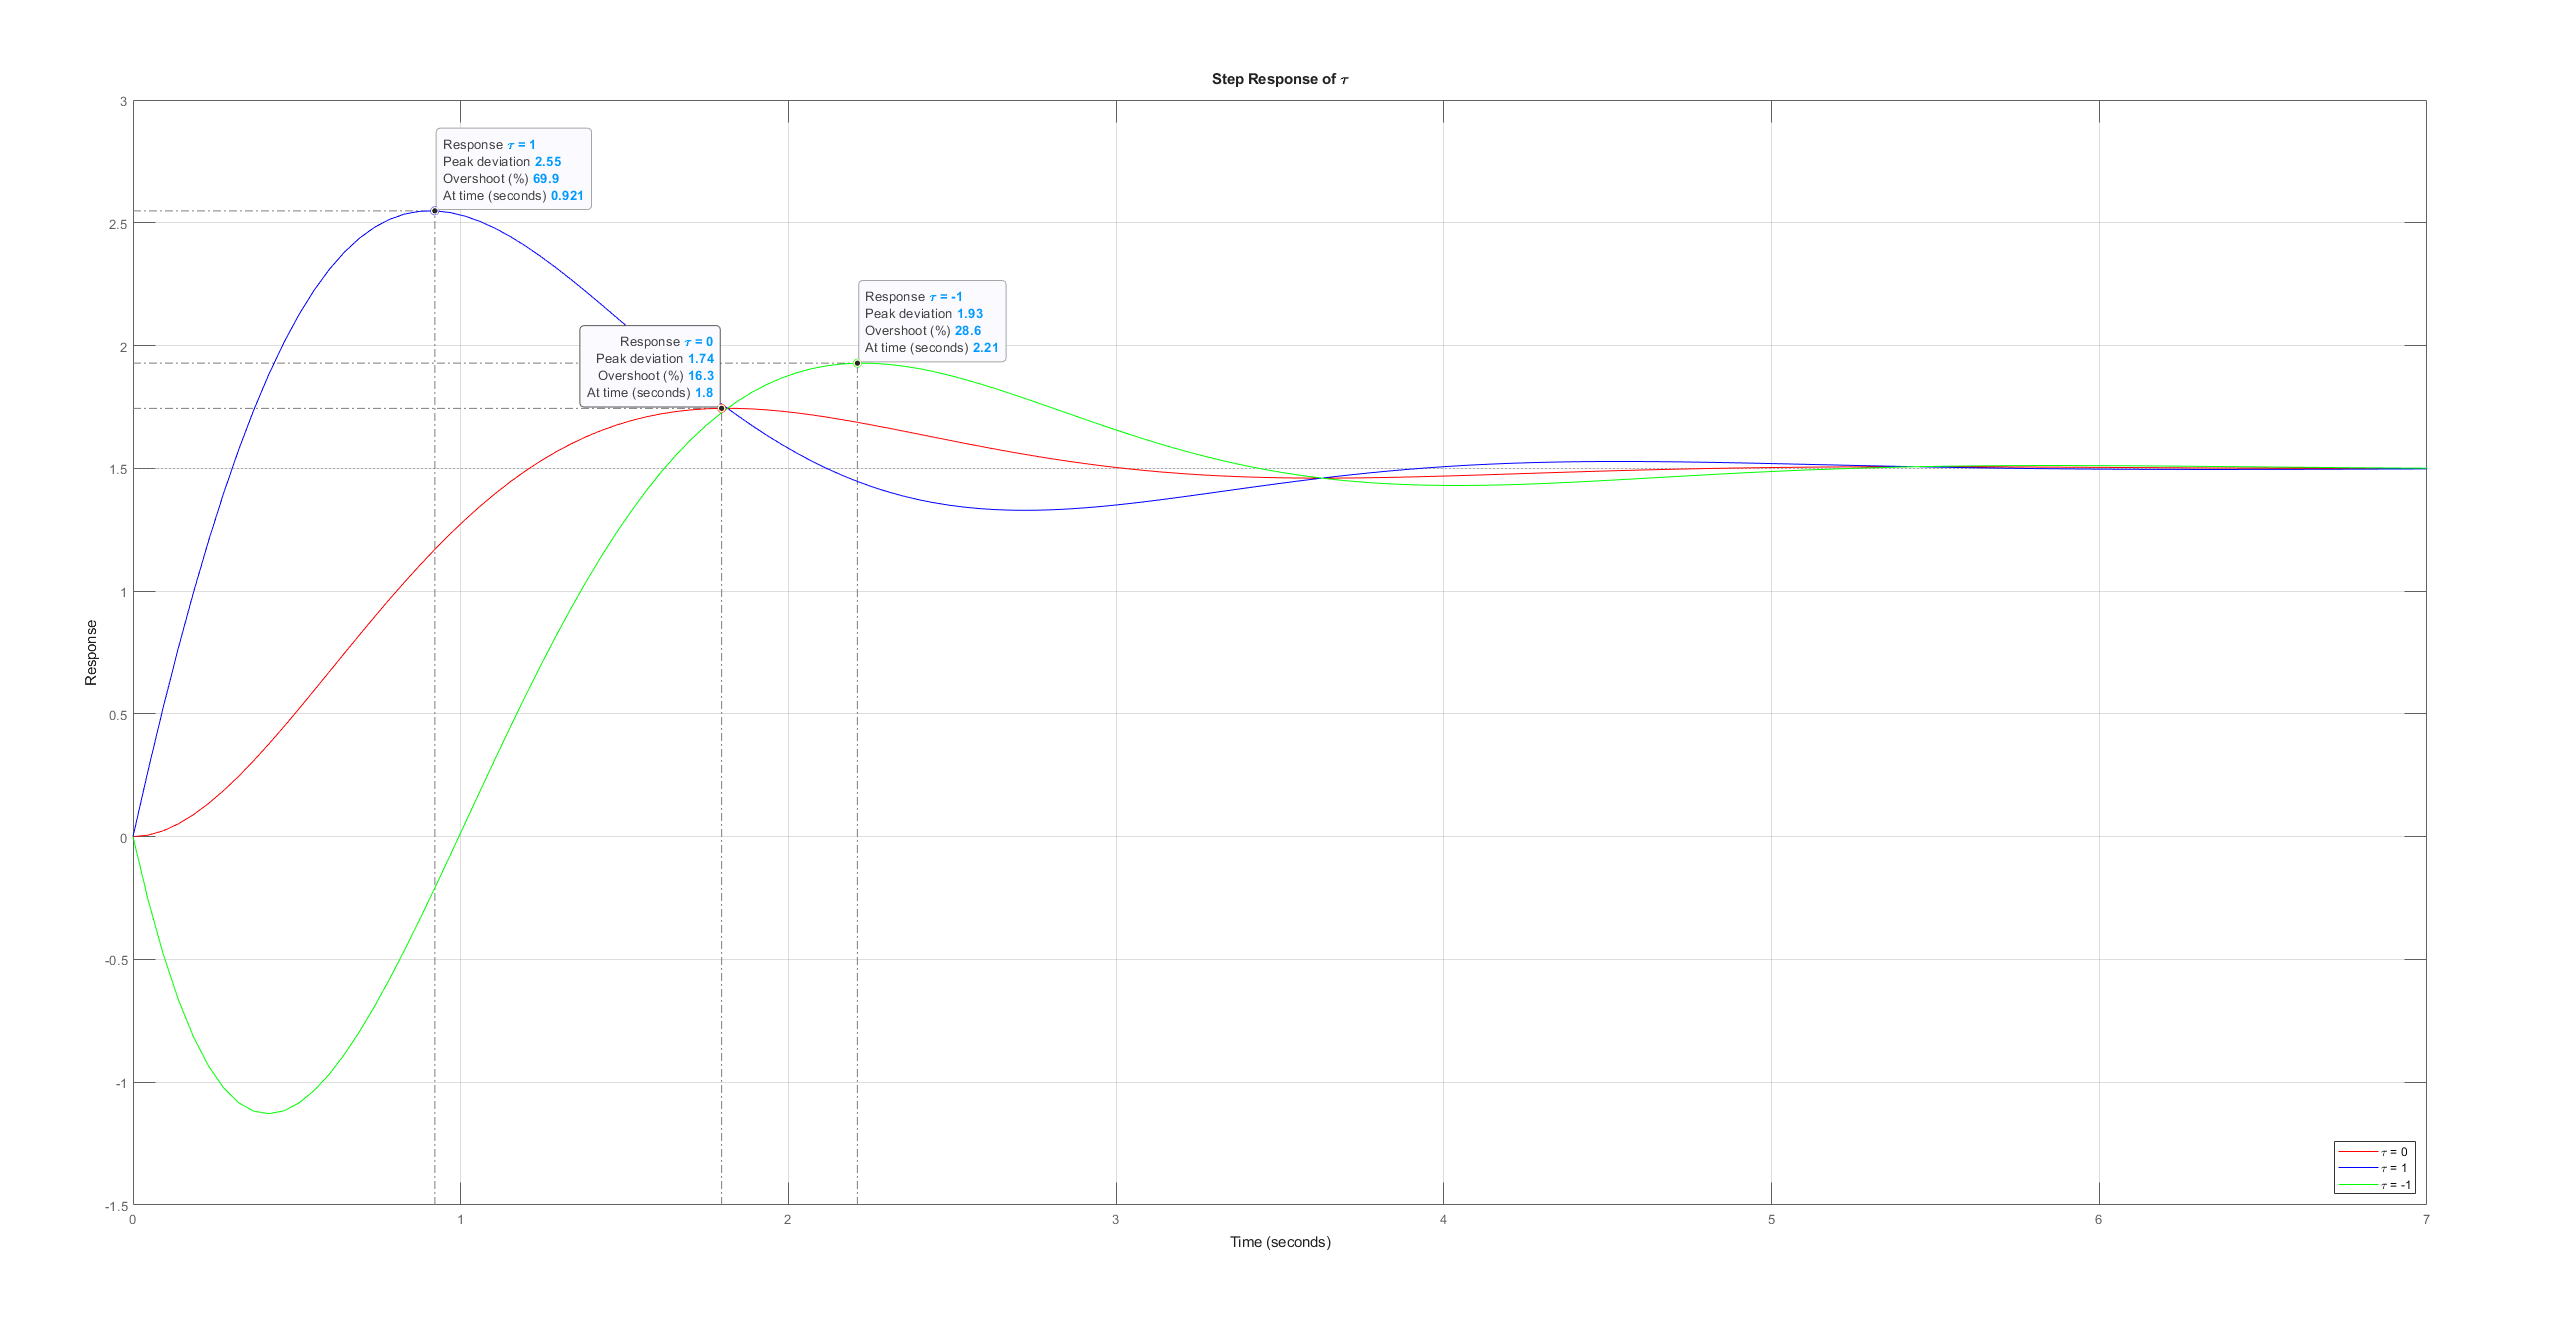
\includegraphics[width=0.8\textwidth]{./images/s01a.png}
		\end{center}
		\caption{Step Response of \( \tau \) with labeled Peak Values and Times}\label{fig:s01a}
	\end{figure}

	\hwkPart{}

	Part B answer

\end{hwkProblem}

\begin{hwkProblem}{2}{}

	\begin{enumerate}
		\item Repeat P01a if instead the denominator of \( \func{G}[s] \) is \( s^{2}+4s+4 \); label the settling times on the graph instead of the peaks
		\item For the \( \tau = 0 \) case, how does the settling time compare with the approximation discussed in the lecture? From the theory, would you expect to see any overshoot in the step response for this case?
		\item For the two cases where \( \tau \neq 0 \), do either exhibit overshoot? If so, how much? Is this overshoot associated with oscillations in the response?
	\end{enumerate}

	\hwkSol{}

	\begin{lstlisting}[language={matlab}, label={lst:s02}, caption={MATLAB code for HW05 P02}]
		denom = s^2 + 4*s + 4;

		figure;
		hold on;
		for j = 1:length(tau)
			G = 6 * (tau(j) * s + 1) / denom;
			step(G,colors(j));
		end

		grid on;
		legend('\tau = 0', '\tau = 1', '\tau = -1', 'Location', 'best');
		title('Step Response');
		xlabel('Time');
		ylabel('Response');
		hold off;
	\end{lstlisting}

	\hwkPart{}

	Part A answer

	\begin{figure}[H]
		\begin{center}
			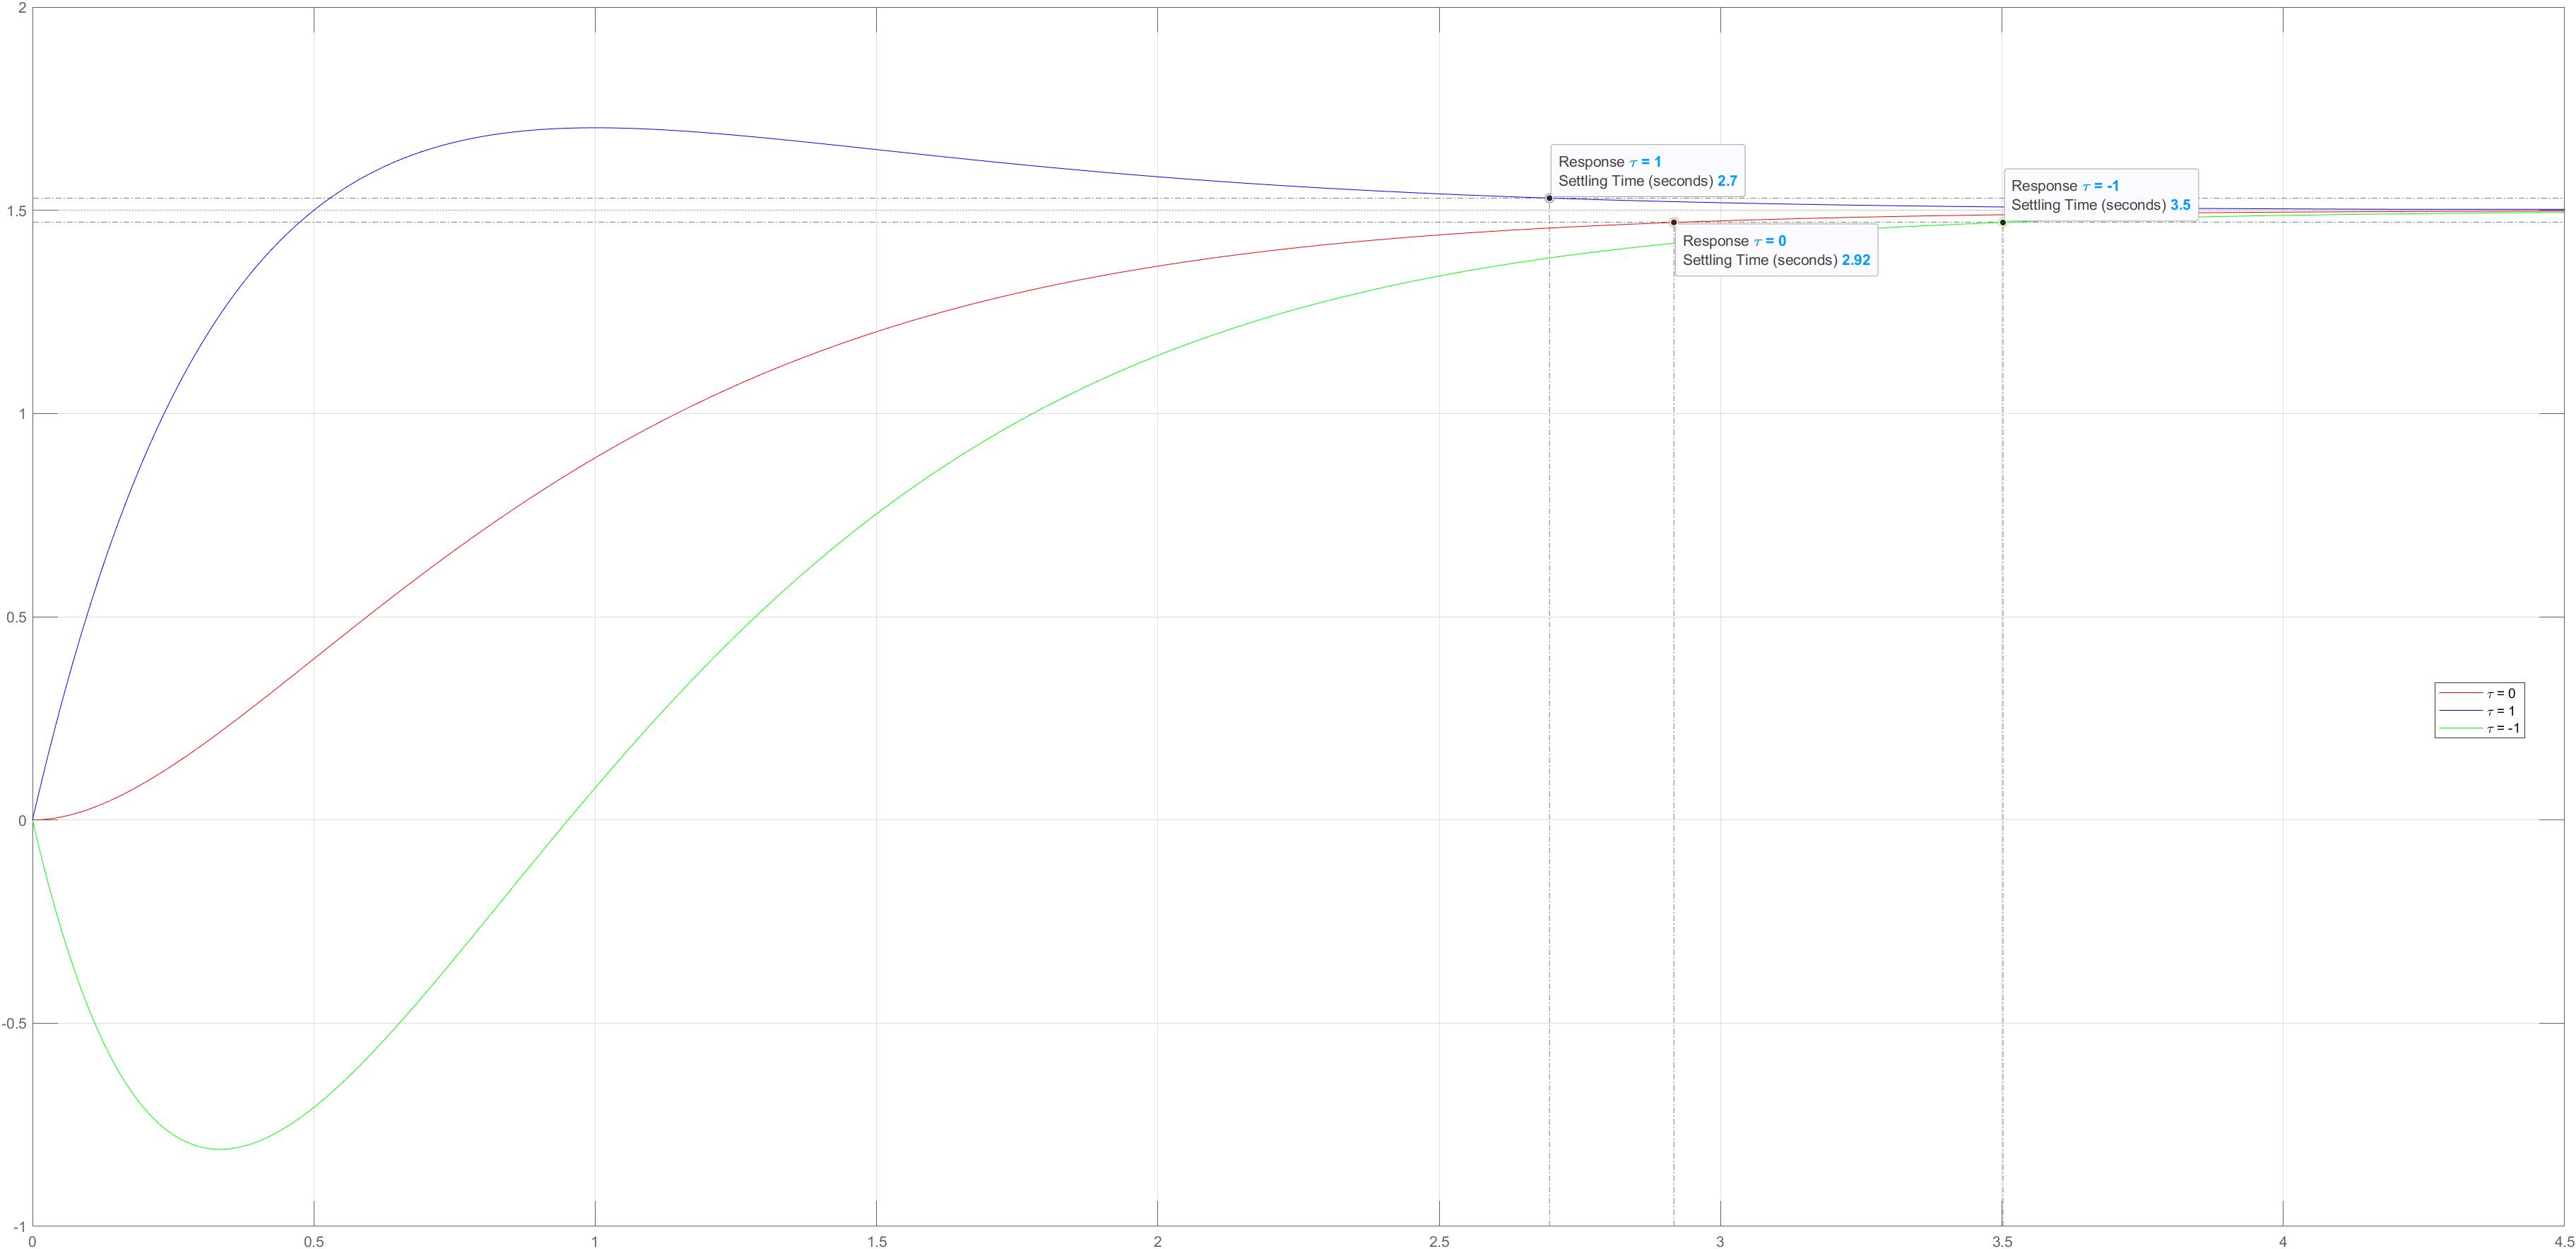
\includegraphics[width=0.8\textwidth]{./images/s02a.png}
		\end{center}
		\caption{Step Response of \( \tau \) with labeled Settling Times}\label{fig:s02a}
	\end{figure}

	\hwkPart{}
	
	Part B answer

	\hwkPart{}

	Part C answer

\end{hwkProblem}

\begin{hwkProblem}{3}{}

	Use MATLAB to obtain the Bode diagrams for the transfer function: \[ G(s)=\frac{5000(s+.02)}{3(2+s)(20+s)^{2}} \].
	\begin{enumerate}
		\item If the input to the system is \(u(t)=\sin (6 t / 10)\), what does the diagram predict the steady-state output of the system will be? Highlight the point(s) on each diagram you use to calculate this.
		\item Analytically verify your result in P03a by explicitly calculating \(G(j \omega),|G(j \omega)|\), and \(\angle G(j \omega)\) for the appropriate value of \(\omega\).
		\item If the input to the system is \(u(t)=2 \sin (70 t+\pi / 4)\), what do you expect the steady-state output of the system will be? Indicate the point(s) on each diagram you use to calculate this. Repeat P03b for this input.
		\item For an input of the form \(u(t)=2 \sin (\omega t)\), approximately what range of frequencies \(\omega\) would result in the largest amplitude oscillations in the steady-state output? Determine from the graph as exactly as possible the actual output amplitude at these frequencies. Verify using the technique in P03b.
		\item For the input in P03d, what value of \(\omega\) will result in the output oscillations lagging the input by \( \qty{90}{\degree} \) ("lag" = negative phase shift)? What will the amplitude of the output oscillations be at this frequency? Use the plot to estimate, then the technique in P03b for precision.
	\end{enumerate}

	\hwkSol{}

	\begin{lstlisting}[language={matlab}, label={lst:s03}, caption={MATLAB code for HW05 P03}]
		G = (5000 * (s + 0.02))/(3 * (2 + s) * (20 + s)^2);
		w = logspace(-3, 3, 10000);
		figure;
		bode(G,w);
		grid on;
		title('Bode Diagram of G(s)');
	\end{lstlisting}

	\hwkPart{}

	Part A answer

	\begin{figure}[H]
		\begin{center}
			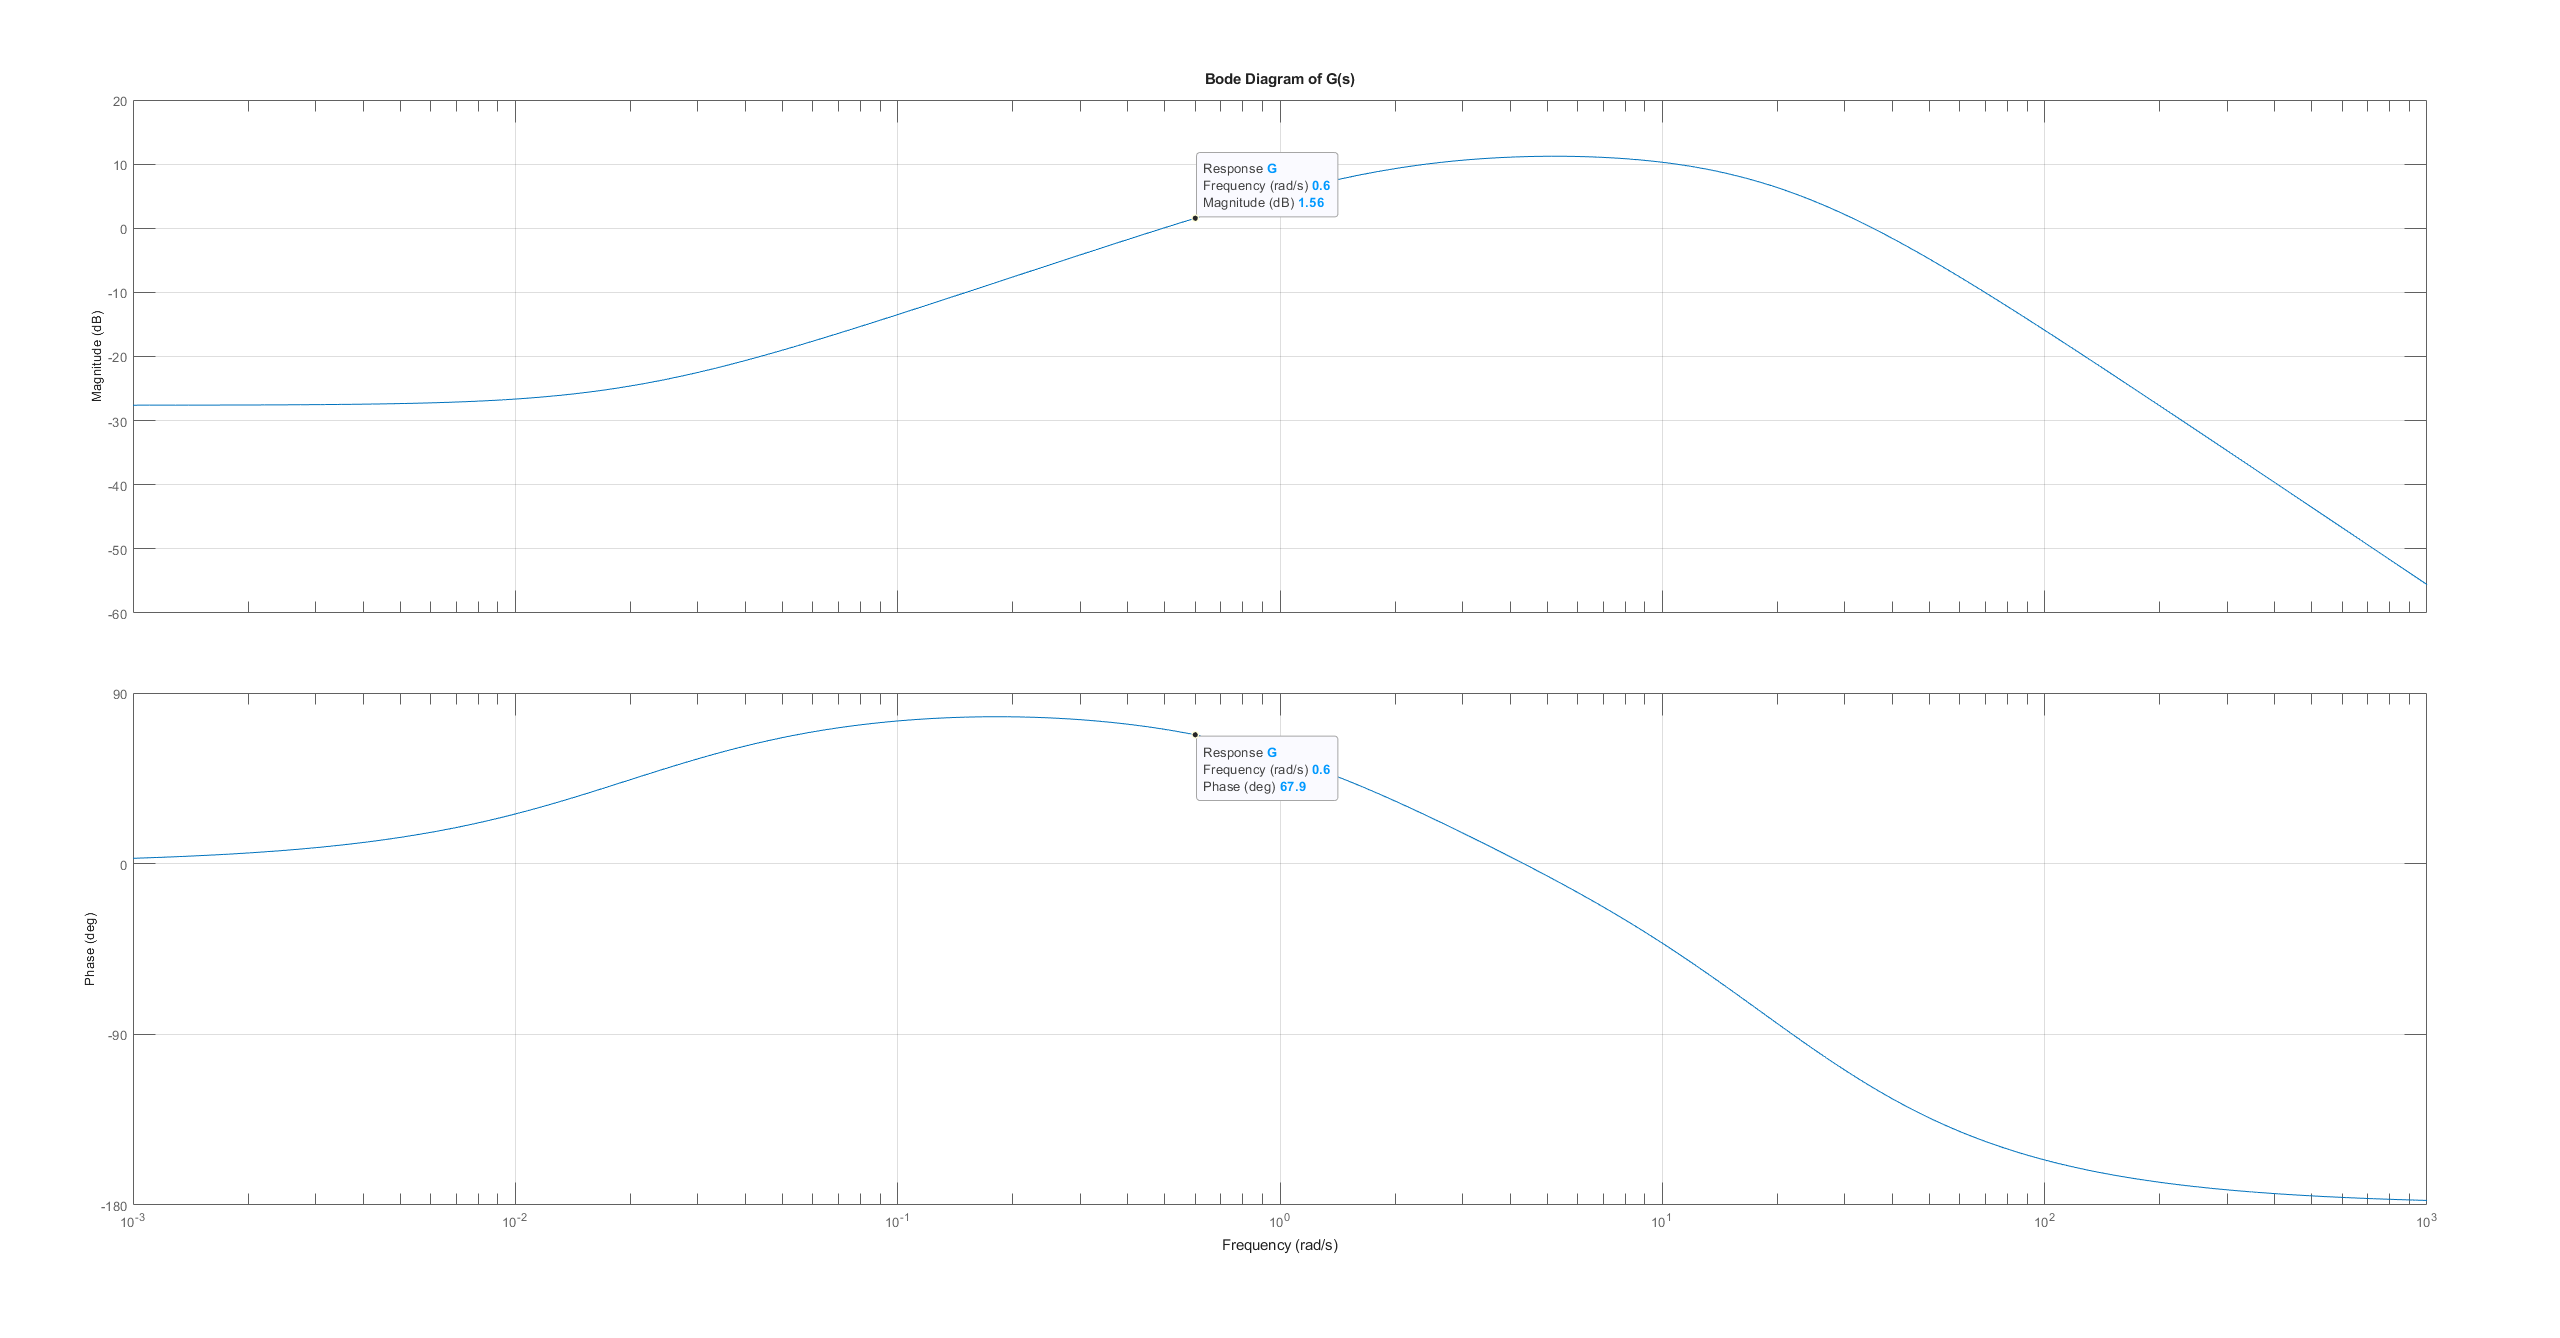
\includegraphics[width=0.8\textwidth]{./images/s03a.png}
		\end{center}
		\caption{Bode Diagrams of \( \func{G}[s] \) with labeled Steady-State Predictions}\label{fig:s03a}
	\end{figure}

	\hwkPart{}
	
	Part B answer

	\hwkPart{}

	Part C answer

	\begin{figure}[H]
		\begin{center}
			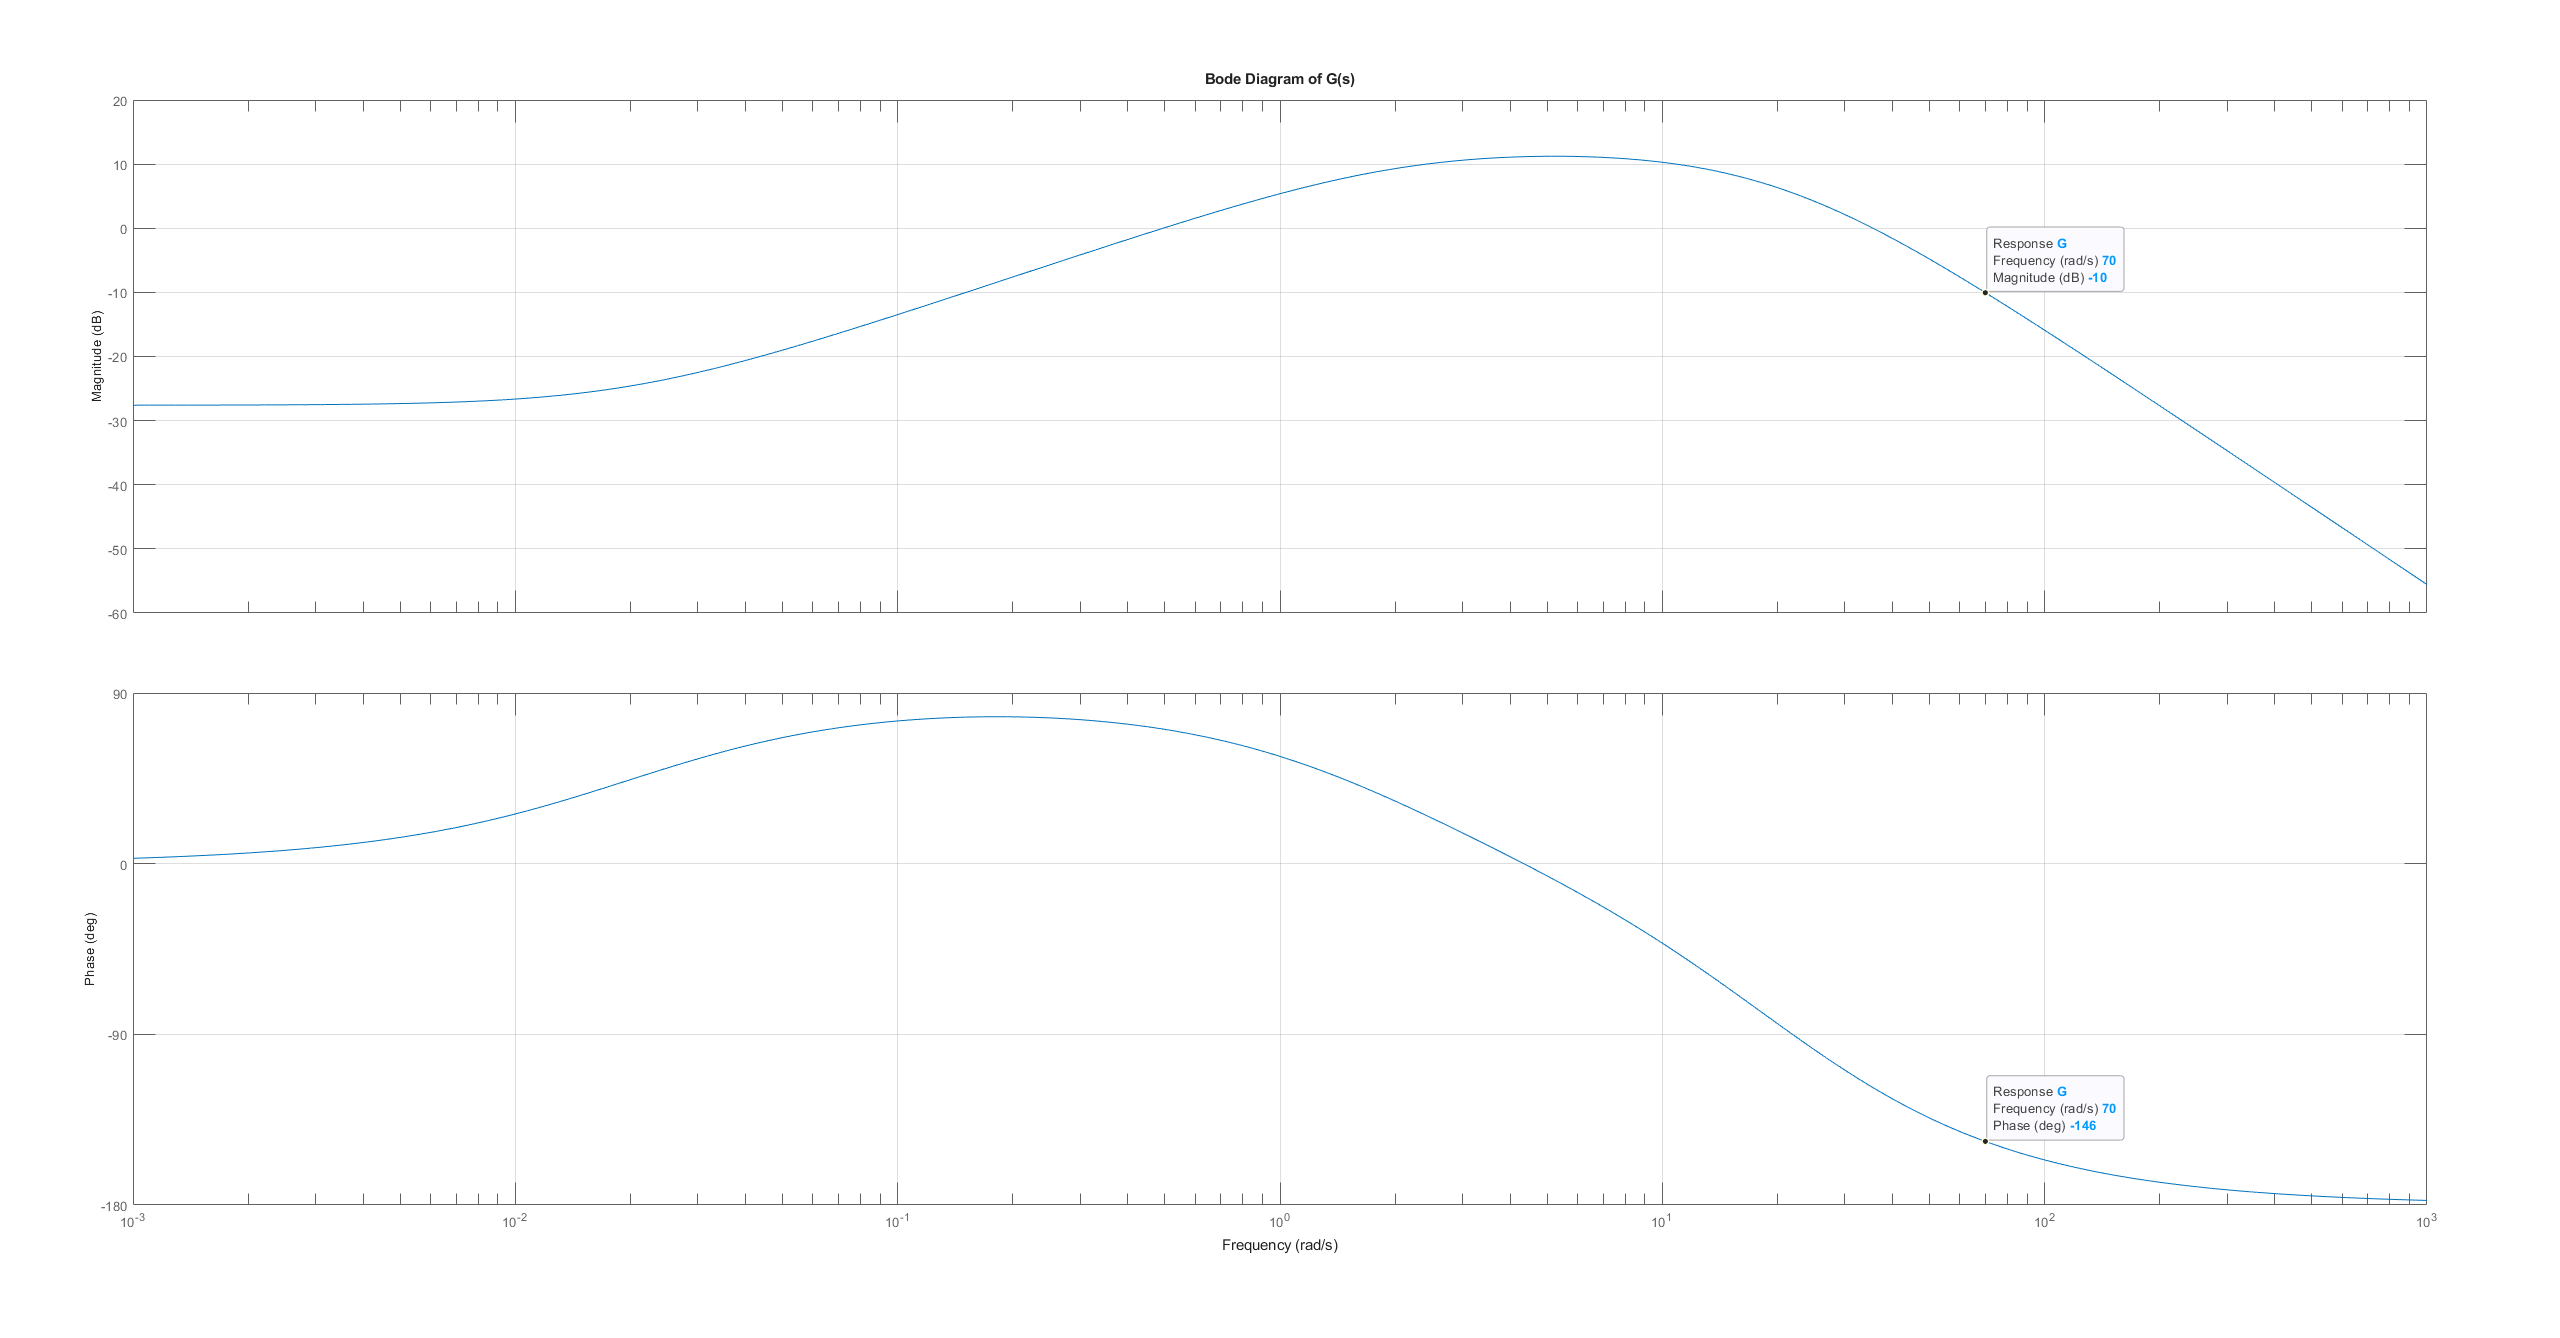
\includegraphics[width=0.8\textwidth]{./images/s03c.png}
		\end{center}
		\caption{Bode Diagrams of \( \func{G}[s] \) with labeled Steady-State Predictions}\label{fig:s03c}
	\end{figure}

	\hwkPart{}

	Part D answer

	\hwkPart{}

	Part E answer

\end{hwkProblem}

\begin{hwkProblem}{4}{}

	\begin{enumerate}
		\item Give the Bode form for the transfer function in P03. Identify the Bode gain numerically. Discuss how and why this gain agrees with the "starting" (low frequency) magnitude shown on the left side of the Bode magnitude plot in P03.
		\item Use the bodemag function in MATLAB to get just the Bode magnitude diagram for the transfer function in P03, put a grid on it, and print out this plot (use orient landscape just before printing to get a plot that fills the page horizontally). Sketch on top of this diagram the straight-line approximation using the technique described in class. Comment on the accuracy of this approximation.
	\end{enumerate}

	\hwkSol{}

	\begin{lstlisting}[language={matlab}, label={lst:s04}, caption={MATLAB code for HW05 P04}]
		f1 = figure;
		bodemag(G);
		grid on;
		orient landscape;
		title('Bode Magnitude Diagram');
	\end{lstlisting}

	\hwkPart{}

	Part A answer

	\hwkPart{}

	Part B answer

	\begin{figure}[H]
		\begin{center}
			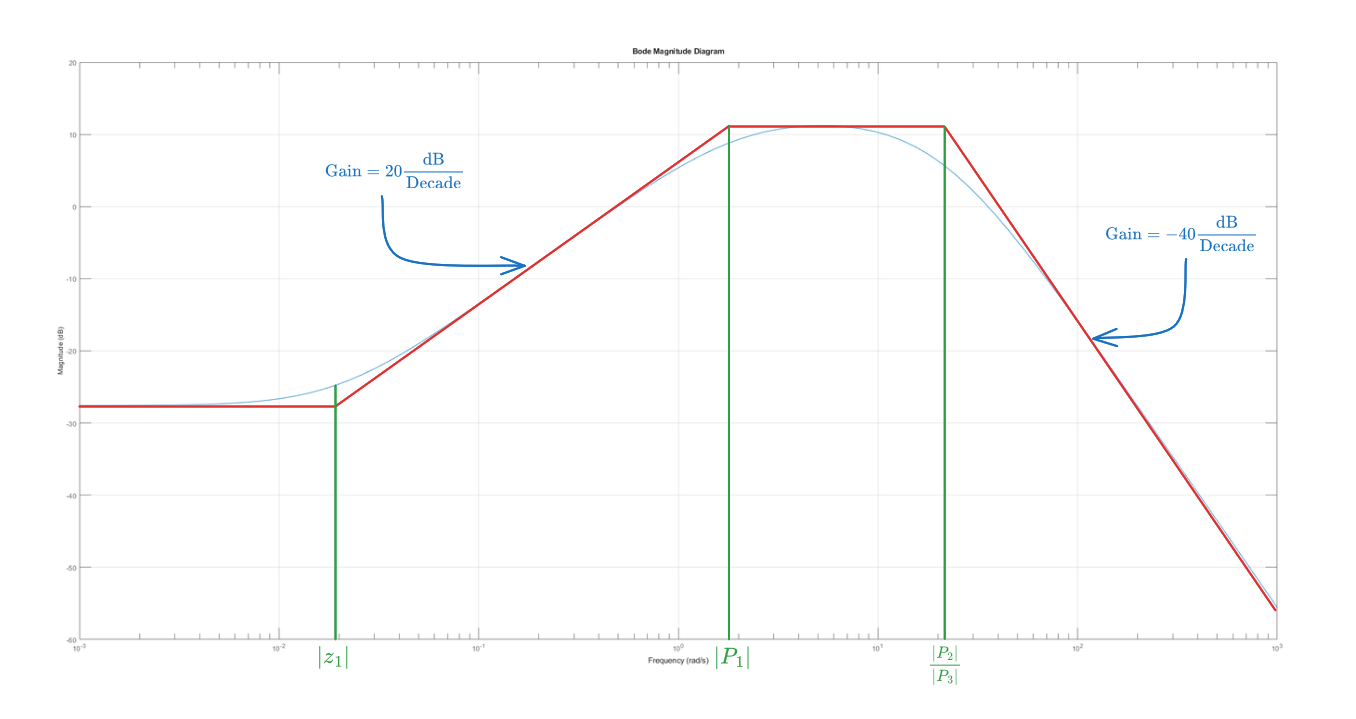
\includegraphics[width=0.8\textwidth]{./images/s04b.png}
		\end{center}
		\caption{Bode Magnitude Diagram of \( \func{G}[s] \) with sketched straight-line approximation}\label{fig:s04b}
	\end{figure}
	
\end{hwkProblem}

\end{document}
